\section{The GX and UX-Method}
\label{sec:gx_ux_method}
UX is a development method, which bases development of a given software product on User Experience (UX).
While we did not follow the UX development method during this project, a paper on user evaluation of a game was based on this development method.
The paper saw shortcomings in the way UX was used to test video games, which inspired the writers to produce their own method, named Gameplay Experience (GX).
We determined that even though it would not be possible for us to carry out the test exactly as described in the paper introducing GX, the way GX thinks about user evaluation of games could be directly translated to this project\cite{gxmethod}.

\subsection{The Three Boxes of GX}
GX splits testing of a game into three boxes.
Each box has its own area of responsibility and goals, which allows testers better clarity of what parts of the game are good, and which are not.
Furthermore, GX offers inspiration and ideas on how to measure the findings of a user evaluation.
Doing a three-way split of the evaluation also ensures that developers can better understand the shortcomings of the games.
As GX shows us, it is not always enough to simply evaluate a game for one set demo

\subsection{Game System Experience}
The Game System Experience is the first box in the GX testing method.
It primarily focuses on testing the game in a specific, software oriented way.
This testing phase does not consider any sort of testing involving a user, rather it strictly concentrates on ensuring that the game runs as expected.
This can for example be done via: Unit Testing, Code Coverage, Stress Testing, Gameplay Metrics and Hardware Tests.
More examples on how a Game System evaluation can be conducted is presented in the paper\cite{gxmethod}.
It is not necessary to go through every kind of test described in the paper to get a useful result, however the more thoroughly the software is tested, the greater the chances are that the program will run as expected.

\subsection{Individual Player Experience}
The Individual Player Experience is the second part of GX.
This is the phase, where tests on a possible user of the game are conducted and recorded.
One of the main challenges with assessing Player Experience is, how does one properly evaluate a players' emotions during playing a game?
Such as, are they frustrated by certain game aspects, are there parts of the game, which the developer wants to be fun and engaging, but ends up being boring for the player?

These things can be difficult to get a clear and unambiguous answer to, but more importantly, for serious games such as ours, where the purpose of the game is to teach, how do we make sure that the player actually learns from playing our game?
These questions belongs to the \textbf{Psycophysiological} aspect of Player Testing.
One proposed solution is to make use of modern sensors such as brain scanners, to see which parts of the brain are activated during certain parts of the game.
For example, assuming the game to test aspires to teach, it would be possible to monitor the sections of the brain that are most used during learning.
If these are highly active, it is an indication that the game manages to teach the player in some form.
The same kind of brain-monitoring test can be done to document engagement or 'fun'.
There are other ways of testing this as well, such as sensors placed on sweat glands, to test levels of 'brain intensity' / taxation and stress.\\

If it is not possible to make an elaborate Psycophysiological test of the player, there are other options available.
These include engaging the player in interviews, questionnaires, software based input logging to document the players activity in the game, player modeling by creating an AI, that simulates a player, and eye tracking technology\cite{gxmethod}.


\subsection{Player Context Experience}
The third and last layer of assessment is often overlooked by game development teams according to \cite{gxmethod}, but is no less important.
This kind of evaluation corresponds to etnographical or location-based testing.
This is typically done on games for mobile platforms, where the context in which the game is played can be very diverse.
The diversity comes from the fact, that mobile games can be played anywhere both on the move to at home on the couch.
Player Context Experience also focuses on how the game is perceived in a multiplayer context, such as what is the social experience from interacting with other players in the game.
Aside from these metrics, it is also possible to do \textbf{Playability Heuristics}, which covers the possibility of having an expert give their review of the game, according to their expert knowledge.
This approach is often the go-to choice by most game developers, because it is cheap and time efficient\cite{gxmethod}.
The layer also include cultural debugging, whose purpose is to ensure, that there are no cultural mishaps between what message the developers wanted to convey, and what the player actually understands based on cultural differences.

\section{Implemented Testing Method}
\label{sec:test_method}

The following section will describe how we set up the testing environment for our users, how we created our test, and how we intend to analyze the data. Finally we will describe the limitations of our testing experience, and why we tested the way we did.

\subsection{The Set-up}

The test will be conducted by requesting a server from the University to host our game, which will then be accessible to the outside world by visiting the website $www.simonjensen.net$.
Making the game available to the entire world ensures, that we have a high chance of getting many people to test our game, which gives the test much more of a quantitative advantage, than necessarily a qualitative advantage.

\subsection{Testing the System - Game System Experience}

We have decided to utilize \textbf{Unit Tests} to check that the code works as intended.
The more code we are able to unit test, the more we ensure a high code coverage on our tests, thus satisfying two schools from the game
experience evaluation box.

\subsection{Testing the Player - Individual Player Experience}

Given the test is going to be accessible to the entire world, a quantitative evaluation seems the most appropriate. Therefore we have chosen to use questionnaires and interviews (/other written feedback) which we request from the users when they have played our game, by following a link to a survey. Furthermore, given we advertise this test on various internet forums, user comments on these will also be taken into consideration for our evaluation.

\subsection{Limitations of our Test Method}

When we take into account the GX method, it is apparent to us, that there are things we cannot test for, since it is both out of scope for this project and the university may not be able to provide the needed technology.
For example, we do not include testing of player context.
It would only be viable for us to test, how well the game plays while on-the-move, in terms of whether the lights and colors on the screen are clear enough.
However hiring an expert in the field to aid with cultural debugging is out of scope, when the target group for this project does not imply cultural differences.
Furthermore, the game in its current state does not work on a mobile platform.

In terms of evaluating the player, it is not possible for us to set up a psycophysiological test, as that would demand access to hardware that we do not currently posses. We have chosen a quantitative testing method over a qualitative method, which means that we will not have direct access to conversations with our testers, and understand in greater depth their issues with the program. Furthermore, we cannot guarantee that every tester, actually fills out the questionnaire. Therefore we are very dependent on, they fill out the survey, after playing the game. In return however, we get a much more informal testing method for our players, and we hope the great accessibility will compensate and uncover the more obvious problems with our software.

\subsection{Questionnaire}

The questionnaire is based around a 'rating-approach', letting people chose between various levels of agreement for each question. We feel this approach is faster for a tester to fill out, and gives more freedom in how they chose to reply. Of course, letting the players entirely describe each answer in detail, is an option as well, but this may be too daunting and time consuming for users, when they are asked to test in this informal and casual way our test-setup suggests.

\begin{figure}[h]
	\centering
		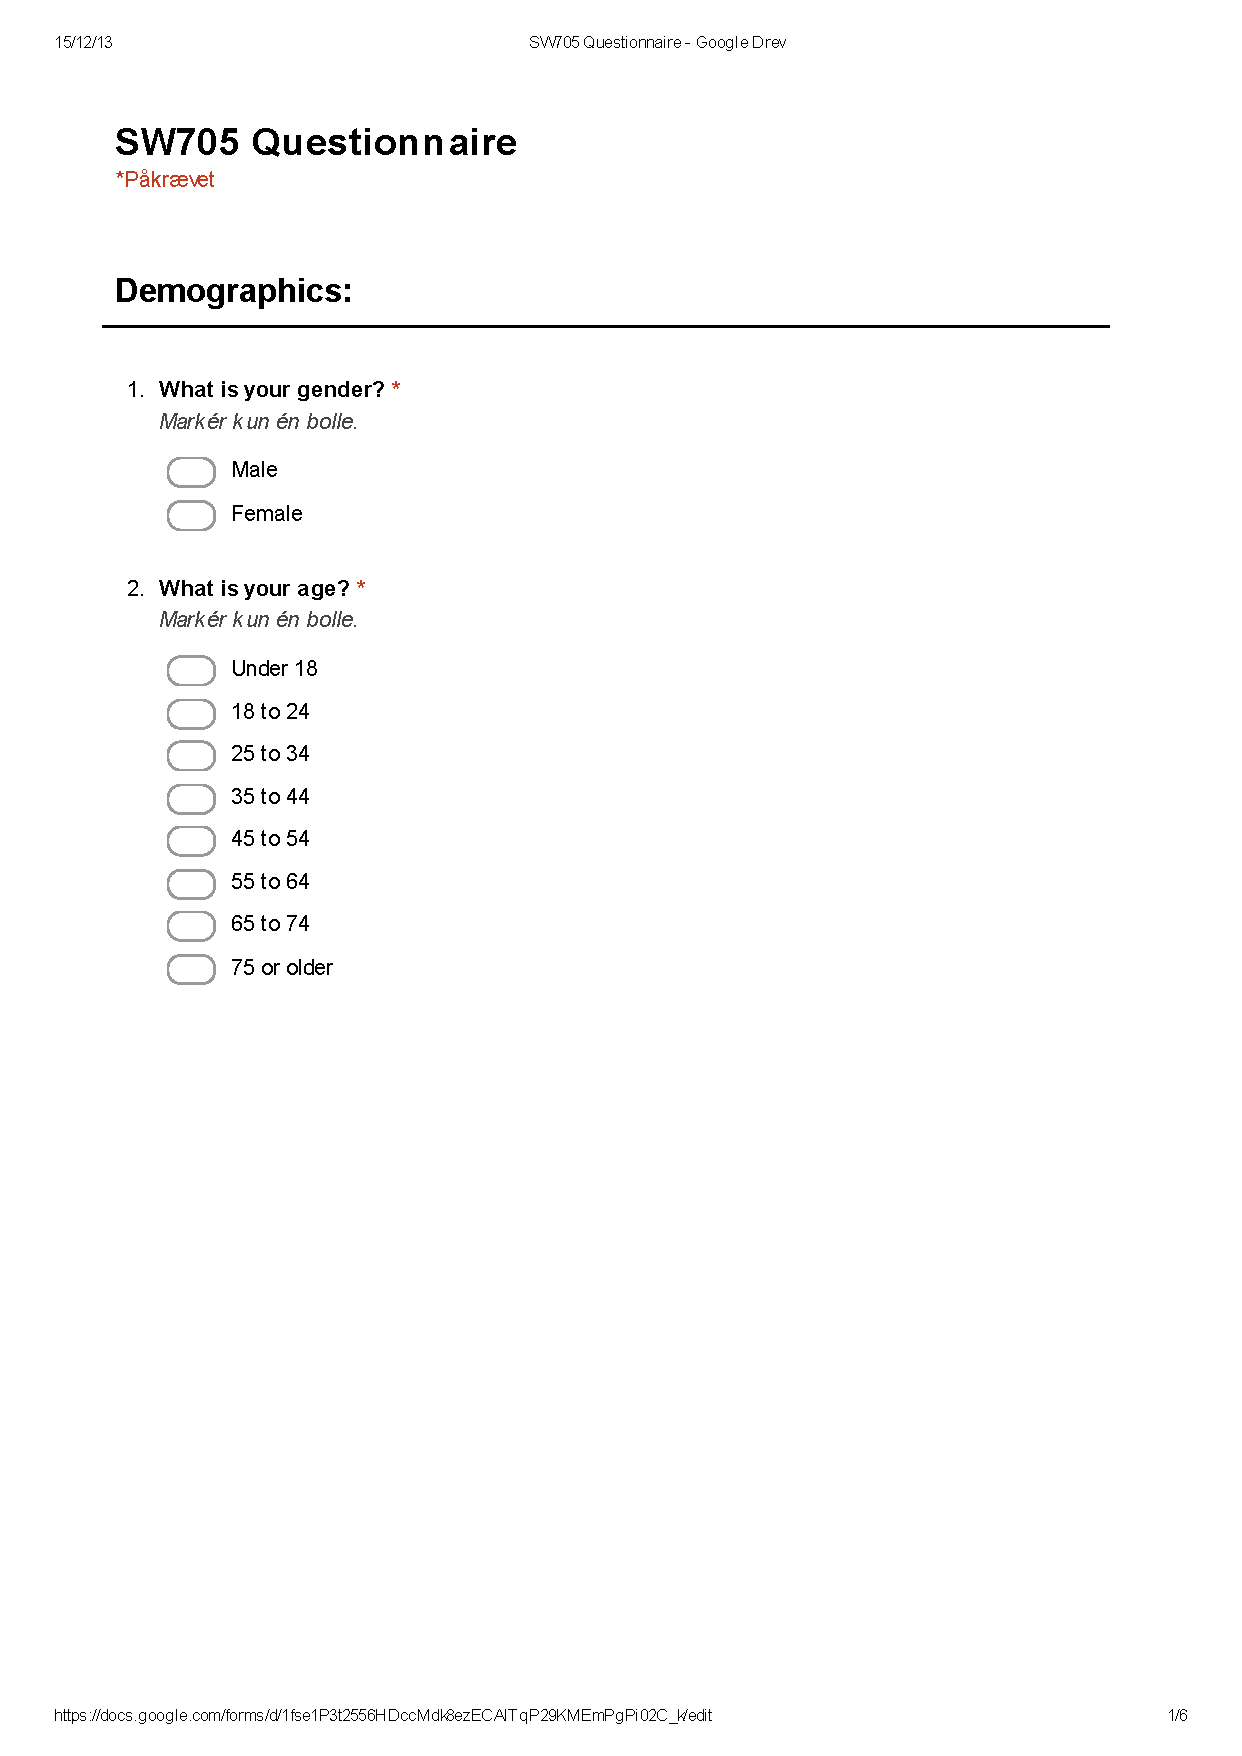
\includegraphics{bib/pdf/SW705 Questionnaire.pdf}
	\caption{The Questionnaire sent to Testers}
	\label{fig:SW705 Questionnaire}
\end{figure}




\subsection{Results}